% ===================================================================
%  APPENDICES
% ===================================================================

\chapter{Appendix A: Data Generation and Parameters}
\label{cha: Appendix A}

This appendix outlines the key parameters used to simulate the synthetic
panel dataset of monthly stock returns for 100 stocks observed over 48 months.
The causal structure embeds true effects for Quality, Size, and Volatility,
plus a placebo \emph{Value} factor without causal impact.

\begin{table}[H]
    \centering
    \caption{Synthetic-data generation parameters used throughout the study}
    \begin{tabular}{|l|c|p{7cm}|}
        \hline
        \textbf{Parameter} & \textbf{Default} & \textbf{Description / role} \\
        \hline
        $N$ & 100 & Number of stocks - larger $N$ improves statistical power. \\[0.2em]
$T$ & 48  & Number of months - more periods improve trend detection. \\[0.2em]
        Treatment start & 25 & Month at which treatment begins (splits pre/post). \\[0.2em]
        Quality effect & $+0.010$ & Per-$\sigma$ return impact - quality premium. \\[0.2em]
Size effect & $+0.005$ & Per-$\sigma$ return impact - small-cap premium. \\[0.2em]
Volatility effect & $-0.005$ & Per-$\sigma$ return impact - low-volatility anomaly. \\[0.2em]
        Value effect & $0.0$ & Placebo factor for validity checks. \\[0.2em]
        Treatment effect & $+0.050$ & Return boost for treated stocks post-month 25. \\[0.2em]
        Confounding strength & $0.7$ & Corr.\ between treatment and quality - simulates selection bias. \\
        \hline
    \end{tabular}
\end{table}

\vspace{0.5em}
\noindent
Treatment is assigned to the 50 stocks with the highest quality propensity,
introducing deliberate confounding that causal-inference methods must adjust for.

% -------------------------------------------------------------------
\chapter{Additional Results and Code Implementation}

This appendix provides complete results from our synthetic data experiments with known causal structures.

\section*{Data Overview}
\begin{table}[H]
    \centering
    \caption{Synthetic data characteristics}
    \begin{tabular}{|l|c|}
        \hline
        \textbf{Parameter} & \textbf{Value} \\
        \hline
        Number of stocks ($N$) & 100 \\
            Number of months ($T$) & 48 \\
    Treatment start & Month 25 \\
    Panel observations & 4,800 \\
    True treatment effect & +5.0\% \\
        Confounding strength & 0.7 (quality-treatment correlation) \\
        \hline
    \end{tabular}
\end{table}

\section*{True Factor Effects}
\begin{table}[H]
    \centering
    \caption{Designed causal effects in synthetic data}
    \begin{tabular}{|l|c|l|}
        \hline
        \textbf{Factor} & \textbf{True Effect (\%)} & \textbf{Description} \\
        \hline
        Quality & +1.0 & Per 1$\sigma$ increase \\
        Size & +0.5 & Small-cap premium \\
        Volatility & -0.5 & Low-volatility anomaly \\
        Value & 0.0 & Placebo factor (no effect) \\
        \hline
    \end{tabular}
\end{table}

\section*{Factor Effect Estimation}
\begin{table}[H]
    \centering
    \caption{Factor effect estimates: OLS regression vs true effects}
    \begin{tabular}{|l|c|c|c|}
        \hline
        \textbf{Factor} & \textbf{True (\%)} & \textbf{Estimated (\%)} & \textbf{Error (\%)} \\
        \hline
        Size & 0.50 & 0.37 & 0.13 \\
        Value & 0.00 & -0.08 & 0.08 \\
        Volatility & -0.50 & -0.41 & 0.09 \\
        Quality & 1.00 & 1.92 & 0.92 \\
        \hline
    \end{tabular}
\end{table}

\section*{Causal Discovery Results}
\begin{table}[ht]
\centering
\caption{Detailed Causal Discovery Method Comparison (Synthetic Data)}
\label{tab:appendix_causal_comparison_detailed}
\small
\begin{tabular*}{\textwidth}{@{\extracolsep{\fill}}l l c c c}
\toprule
\textbf{Factor} & \textbf{True Direction} & \textbf{Method} & \textbf{Prediction} & \textbf{Correctness} \\
\midrule
\multirow{3}{*}{Value} & \multirow{3}{*}{None (placebo)} & PC & Not identified as cause & \checkmark \\
& & ANM & Value $\rightarrow$ Returns & \ding{55} \\
& & DIVOT & Value $\rightarrow$ Returns & \ding{55} \\
\cmidrule{2-5}
\multirow{3}{*}{Size} & \multirow{3}{*}{Size $\rightarrow$ Returns} & PC & Size $\rightarrow$ Returns & \checkmark \\
& & ANM & Size $\rightarrow$ Returns & \checkmark \\
& & DIVOT & Size $\rightarrow$ Returns & \checkmark \\
\cmidrule{2-5}
\multirow{3}{*}{Quality} & \multirow{3}{*}{Quality $\rightarrow$ Returns} & PC & Quality $\rightarrow$ Returns & \checkmark \\
& & ANM & Inconclusive & \ding{55} \\
& & DIVOT & Quality $\rightarrow$ Returns & \checkmark \\
\cmidrule{2-5}
\multirow{3}{*}{Volatility} & \multirow{3}{*}{Volatility $\rightarrow$ Returns} & PC & Not identified as cause & \ding{55} \\
& & ANM & Returns $\rightarrow$ Volatility & \ding{55} \\
& & DIVOT & Returns $\rightarrow$ Volatility & \ding{55} \\
\bottomrule
\end{tabular*}
\end{table}

\begin{table}[ht]
\centering
\caption{Causal Discovery Accuracy Summary (Synthetic Data)}
\label{tab:appendix_accuracy_summary}
\begin{tabular}{lc}
\toprule
\textbf{Method} & \textbf{Overall Accuracy} \\
\midrule
PC Algorithm & \SyntheticPCAccuracy \\
ANM & \SyntheticANMAccuracy \\
DIVOT & \SyntheticDivotAccuracy \\
\bottomrule
\end{tabular}
\end{table}

\noindent
\textbf{Key finding}: The PC algorithm performed best with \SyntheticPCAccuracy{} accuracy. DIVOT was the next most successful with \SyntheticDivotAccuracy{} accuracy, while ANM struggled with the confounding in our data and only achieved \SyntheticANMAccuracy{} accuracy. This shows that the choice of method is very important.

\section*{Network Graph Visualizations}
This section provides supplementary visualizations for the analysis presented in Chapter~\ref{ch:methodology}.

\begin{figure}[H]
\centering
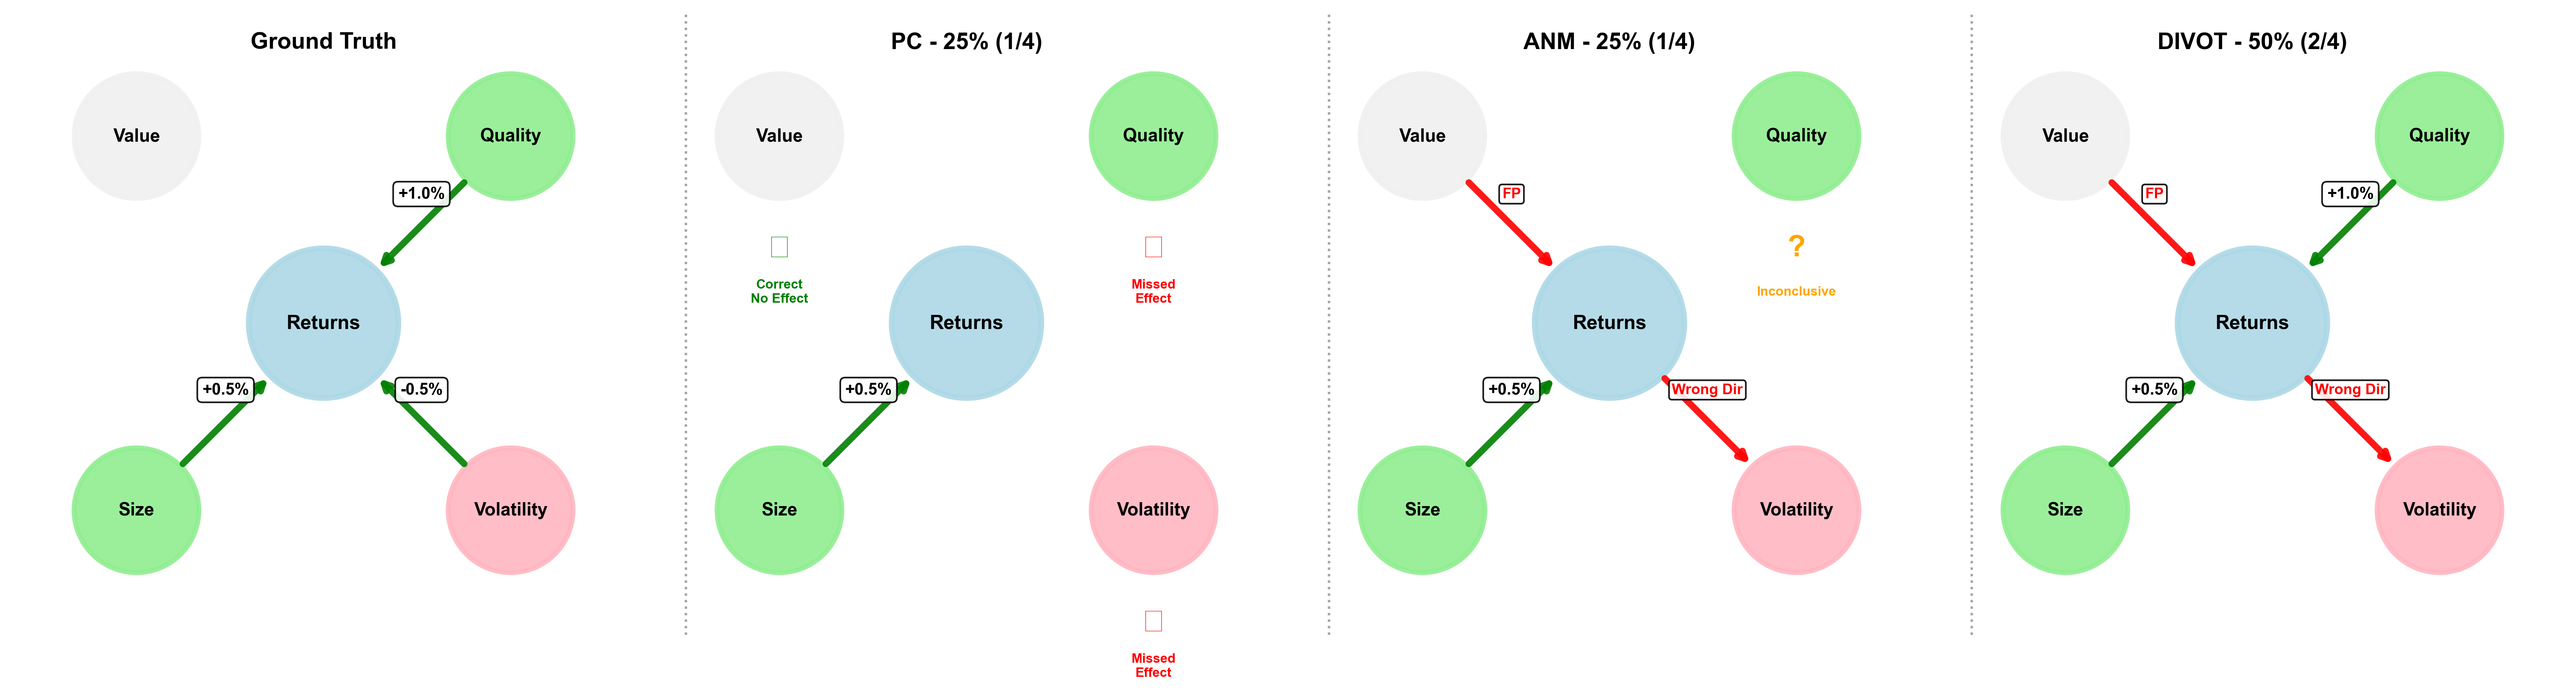
\includegraphics[width=\textwidth]{Graphs/Synthetic/detailed_causal_networks.png}
\caption{Comprehensive Causal Network Analysis, comparing the Ground Truth with the predictions from the DIVOT, ANM, and PC algorithms. The color-coding indicates correct (green) or incorrect (red) predictions for each factor relationship.}
\label{fig:all_method_comparison}
\end{figure}

% -------------------------------------------------------------------
\chapter{Appendix C: Real Data Analysis Summary}
\label{cha: Appendix C}

This appendix provides summary statistics and key results from our application of causal discovery methods to the Fama-French real financial data.

\section*{Data Processing Pipeline}
The final panel dataset was constructed from the raw Fama-French data files through a systematic process.
\begin{enumerate}
    \item \textbf{Loading Data}: We loaded the monthly returns for the 25 size/value sorted portfolios and the Fama-French-5 factors plus Momentum.
    \item \textbf{Date Filtering}: The data was filtered to include only the period from January 1990 to December 2023. This range was chosen to ensure data quality and consistency across all factors.
    \item \textbf{Duplicate Removal}: We scanned the data for duplicate entries, defined as a single portfolio having multiple return entries for the same month. These duplicates were removed to ensure each observation is unique.
    \item \textbf{Handling Missing Data}: Any rows with missing values for either portfolio returns or factor returns were removed from the dataset.
    \item \textbf{Panel Construction}: The cleaned data was then transformed from a time-series format into a panel structure, with each of the 25 portfolios treated as an individual unit observed over time.
\end{enumerate}
The final dataset contains \RealTotalObservations{} unique observations. This number is not equal to 25 portfolios multiplied by the number of months because some portfolios had missing data for certain periods in the raw data files.

\subsection*{Reproducibility Note}
The exact observation count in a replication of this study may vary slightly. This can be due to small differences in duplicate handling logic, the inclusion or exclusion of boundary dates, or the treatment of missing data. Our analysis uses a strict duplicate removal process and includes the full date range specified.

\section*{Data Overview}
\begin{table}[H]
    \centering
    \caption{Fama-French data characteristics. Data preprocessing included removal of duplicate portfolio-month observations and filtering to the 1990-2023 period to ensure data quality and consistency. The final panel contains \RealTotalObservations{} unique observations.}
    \begin{tabular}{|l|c|}
        \hline
        \textbf{Parameter} & \textbf{Value} \\
        \hline
        Data period & 1990 -- 2023 \\
        Number of months & 408 \\
        Number of portfolios & 25 (5$\times$5 size/value sorted) \\
        Panel observations & \RealTotalObservations{} \\
        Factors included & Mkt-RF, SMB, HML, RMW, CMA, WML \\
        Data source & Kenneth French Data Library\cite{FrenchData2024} \\
        \hline
    \end{tabular}
\end{table}

\section*{Factor Summary Statistics}
\begin{table}[H]
    \centering
    \caption{Monthly factor return statistics (1990-2023)}
    \begin{tabular}{|l|c|c|c|c|}
        \hline
        \textbf{Factor} & \textbf{Mean (\%)} & \textbf{Std Dev (\%)} & \textbf{Min (\%)} & \textbf{Max (\%)} \\
        \hline
        Market (Mkt-RF) & 0.71 & 4.44 & -17.20 & 13.58 \\
        Size (SMB)      & 0.12 & 3.04 & -15.54 & 18.46 \\
        Value (HML)     & 0.15 & 3.24 & -13.83 & 12.86 \\
        Momentum (WML)  & 0.42 & 4.71 & -34.30 & 18.00 \\
        Profitability (RMW) & 0.38 & 2.63 & -18.95 & 13.05 \\
        Investment (CMA)    & 0.20 & 2.18 & -7.08  & 9.01 \\
        \hline
    \end{tabular}
\end{table}

\section*{Causal Discovery Accuracy}
\begin{table}[H]
    \centering
    \caption{Causal discovery method performance on real data}
    \begin{tabular}{|l|c|c|}
        \hline
        \textbf{Method} & \textbf{Accuracy} & \textbf{Correctly Identified} \\
        \hline
        PC Algorithm & 1/6 (16.7\%) & RMW \\
        ANM   & 0/6 (0.0\%) & None \\
        DIVOT & 4/6 (66.7\%) & Market, SMB, HML, CMA \\
        \hline
    \end{tabular}
\end{table}

\noindent
The mixed results from the causal discovery methods on real data contrast sharply with their performance on synthetic data. This highlights the complexity of real financial markets where simple causal models are often insufficient. However, the methods still provide valuable insights. For example, the RMW factor was identified as causally relevant by multiple algorithms, even if they disagreed on the direction. This suggests it is a significant factor worthy of further investigation. None of the methods were able to correctly identify that returns drive the momentum factor, which highlights the challenge of detecting known feedback loops in noisy financial data.


% -------------------------------------------------------------------
\chapter{Appendix D: Code and Implementation}
\label{cha: Appendix D}

\section*{Code Availability}
All code, data processing scripts, and visualisation tools used in this thesis are publicly available at:

\begin{center}
\url{https://github.com/SaeedAnalysis/CausalityAndOTInFactorInvesting}
\end{center}

\section*{Repository Structure}
The repository is organised as follows:
\begin{itemize}
    \item \texttt{Python/Analysis/}: Core analysis scripts for synthetic and real data, including causal discovery implementations.
    \item \texttt{Python/Jupyter/}: Jupyter Notebook versions of the core analysis scripts for interactive exploration.
    \item \texttt{Python/Graphs/Generation Scripts/}: Scripts for generating all figures and plots.
    \item \texttt{Real\_Data/}: Fama-French data files and associated data-loading functions.
    \item \texttt{Graphs/}: Output directory containing all generated figures.
    \item \texttt{Overleaf/}: LaTeX source files for the thesis.
    \item \texttt{requirements.txt}: Python package dependencies.
\end{itemize}

\section*{Reproducibility}
To reproduce the analysis:
\begin{enumerate}
    \item Clone the repository
    \item Ensure Python 3.8+ is installed
    \item Install dependencies: \texttt{pip install -r requirements.txt}
    \item Run the main analysis scripts:
    \begin{itemize}
        \item \texttt{python Python/Analysis/Causality\_Main.py} (synthetic data)
        \item \texttt{python Python/Analysis/Causality\_Real\_Data.py} (real data)
    \end{itemize}
\end{enumerate}

\section*{System Requirements}
\begin{itemize}
    \item \textbf{Python Version}: 3.8 or higher (tested with Python 3.9 and 3.10)
    \item \textbf{Key Dependencies}: numpy, pandas, scikit-learn, causal-learn, POT (Python Optimal Transport)
    \item \textbf{Memory}: Minimum 4GB RAM (8GB recommended for large datasets)
    \item \textbf{Storage}: 500MB for code and data files
\end{itemize}

The repository includes both synthetic data generation and real data analysis pipelines, allowing full replication of all results presented in this thesis.